\documentclass[12pt]{article}
\usepackage[utf8]{inputenc}
\usepackage{graphics}
\usepackage{graphicx}

\title{Release plan}
\author{Thomas van Dongen, Koen Schilders}
\date{7 februari 2018}

\begin{document}

\begin{titlepage}
\maketitle
\end{titlepage}

\begin{figure}
	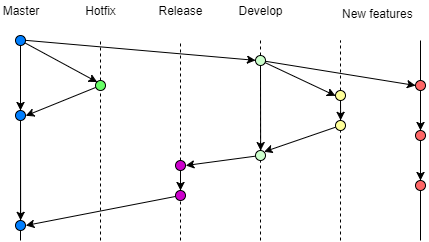
\includegraphics[width=\textwidth]{images/SOP6_Release.png}
	\caption{Het releaseplan.}
\end{figure}

\section{Omschrijving per branch}
\subsection{Master}
De master is de branch waar een geteste releases staan.
\subsection{Hotfix}
Als er een ernstige bug gevonden is in de master branch is het nodig om deze direct op te lossen. Een hotfix dient dan in de hotfix branch gemaakt te worden. Hiervoor wordt de build van de master gepulled, en een hotfix gemaakt. Vervolgens wordt deze naar de master gepushed als nieuwe versie.
\subsection{Release}
Todo
\subsection{Develop}
De develop branch wordt gebruikt als start punt voor het ontwikkelen van nieuwe features. Er wordt vanaf deze branch een nieuwe branch gemaakt en daar wordt verder op gewerkt. Er wordt dus nooit ontwikkeld op deze branch.
\subsection{New features}
Voor elke nieuwe feature wordt een nieuwe branch gemaakt.

\end{document}